\documentclass[11pt]{article}
\usepackage[margin=1in]{geometry}
\usepackage{amsmath,amssymb,amsthm}
\usepackage{tikz}
\usetikzlibrary{arrows.meta,positioning,calc}
\usepackage{graphicx}
\usepackage{enumitem}
\usepackage{booktabs}
\usepackage{xcolor}
\usepackage[hidelinks]{hyperref}

\graphicspath{{./}}
\setlength{\parindent}{0pt}
\setlength{\parskip}{5pt}

\newtheorem{theorem}{Theorem}
\newtheorem{lemma}{Lemma}

\definecolor{brass}{HTML}{94690C}
\definecolor{ink}{HTML}{20221E}
\tikzset{
  vtx/.style={circle, draw, thick, minimum size=7mm, inner sep=0pt, font=\small\bfseries, fill=white},
  box/.style={draw, thick, rounded corners=2pt, minimum width=17mm, minimum height=7mm, font=\small, fill=white},
  flow/.style={-{Stealth[length=2mm]}, thick}
}

\title{\vspace{-1.2cm}\textbf{Scheduling a Pool Tournament with Graph Theory}\\
\large A one-factorization round robin, calibrated Elo simulation, and seeded knockouts}
\author{Ayro Escobar \\ CS 4302 Mathematics of Computing, UT Dallas}
\date{}

\begin{document}
\maketitle
\vspace{-1.0cm}

\begin{abstract}
\noindent This project builds and simulates a complete eight ball tournament and,
more importantly for this course, exposes the discrete mathematics behind every
scheduling decision. Modeling the field as the complete graph $K_n$ turns the two
central questions, who plays whom and in what order, into classical structures: a
round robin becomes a one-factorization of $K_n$, a knockout becomes a seeded
binary tree, and a fair rating becomes an Elo model. I give the circle method with
a full correctness proof (it works because $2$ is a unit modulo the odd number
$n-1$), calibrate the match simulation so its outcomes match the Elo odds exactly,
build both single and double elimination knockouts with their match count
arguments, and analyze the carry-over effect, where a recent theorem shows the
circle method is the most unbalanced schedule possible. Every claim is verified,
either by a live panel that recomputes it from the generated schedule or by a test
suite of roughly $108{,}000$ assertions run against the exact shipped code.
\end{abstract}

\section{Introduction}

The University of Texas at Dallas Student Union has pool tables, and a recurring
question is how to run a fair, skill based tournament there. Stripped of the game
itself, the problem is purely combinatorial. Draw each player as a vertex and each
match as an edge, and the tournament becomes a graph. The scheduling questions then
become questions that discrete mathematics answers cleanly and provably:

\begin{itemize}[nosep,leftmargin=1.4em]
  \item A round robin, where everyone plays everyone, is the complete graph $K_n$.
  \item Assigning matches to rounds so that no player is in two at once is an edge
        coloring, equivalently a one-factorization, of that graph.
  \item A single elimination bracket is a binary tree.
  \item Rating and seeding players fairly is handled by the Elo system.
\end{itemize}

The project began as a real event. I built the system so a group of friends and I
could run a proper seeded tournament on those tables, and I trialed it with three
or four friends to exercise the roster entry and the opening rounds. A full live
bracket did not survive the summer: between everyone's internships there was never
a night with the whole field free. So the version presented here exercises the
system by simulation instead. The app plays complete tournaments with rated odds,
which turned out to be the better showcase for the mathematics anyway, since a
simulated field can be rerun, resized, and pushed to thirty players on demand,
while one evening of live pool demonstrates a single schedule once.

The deliverable is a single self contained web page (no build step, no external
libraries, no stored data) that reads a roster of $4$ to $30$ players, generates
the schedule, plays every match with rated odds, and crowns a champion, while a
side panel and an interactive walkthrough display the mathematics as it happens.
This report presents that mathematics and the reasoning behind each design choice.

\section{The graph model and the round robin}

\subsection{Counting the matches}

With $n$ players, a full round robin plays every unordered pair once. In $K_n$
every vertex has degree $n-1$, so by the handshake lemma
\[
|E(K_n)| = \frac{1}{2}\sum_{v}\deg(v) = \frac{n(n-1)}{2},
\]
which is the total number of matches. For $n=8$ this is $28$.

\subsection{A round is a perfect matching, a schedule is a one-factorization}

A single round is played simultaneously, so no player may appear twice. In graph
terms a round is a \emph{perfect matching} of $K_n$, also called a one-factor: a
set of edges meeting every vertex exactly once, hence $n/2$ matches. A schedule
that plays every match once partitions the edge set of $K_n$ into rounds, that is,
into perfect matchings. Such a partition is a \emph{one-factorization}:
\[
E(K_n) = M_1 \cup M_2 \cup \dots \cup M_{n-1}, \qquad M_i \text{ pairwise edge disjoint perfect matchings.}
\]
So building a fair round robin schedule is exactly the problem of one-factorizing
$K_n$. The construction has a long history: Kirkman first built one-factorizations
of complete graphs in 1847, and the rotating circle arrangement appears in Lucas
in 1883.

\subsection{The circle method}

Fix one player in a seat that never moves. Arrange the other $n-1$ players on a
ring. Each round, pair the two players across the ring from each other; then rotate
the ring one seat and repeat, for $n-1$ rounds. Figure~\ref{fig:kn} shows $K_6$
with the first round's matching highlighted.

\begin{figure}[h]
\centering
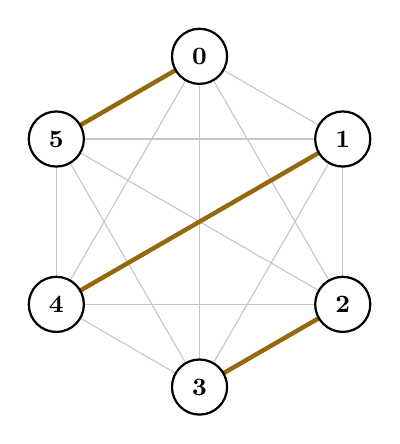
\begin{tikzpicture}[scale=1.0]
  \foreach \i/\ang in {0/90,1/30,2/-30,3/-90,4/-150,5/150} \coordinate (v\i) at (\ang:2.1);
  % all edges light
  \foreach \i in {0,...,5} \foreach \j in {0,...,5} { \ifnum\i<\j \draw[gray!45,thin] (v\i)--(v\j); \fi }
  % round 1 matching: 0-5, 1-4, 2-3
  \draw[brass,line width=1.6pt] (v0)--(v5);
  \draw[brass,line width=1.6pt] (v1)--(v4);
  \draw[brass,line width=1.6pt] (v2)--(v3);
  \foreach \i in {0,...,5} \node[vtx] at (v\i) {\i};
\end{tikzpicture}
\caption{$K_6$ with round 1 of the circle method (the perfect matching
$\{0,5\},\{1,4\},\{2,3\}$) in brass. The five rounds together use all $15$ edges
exactly once, a one-factorization of $K_6$.}
\label{fig:kn}
\end{figure}

The construction is short, but why it is correct is the mathematically interesting
part, and the part a presenter should be able to give unaided.

\begin{theorem}[Correctness of the circle method]
For even $n$, the circle method schedules every pair of players exactly once in
$n-1$ rounds.
\end{theorem}

\begin{proof}
Number the ring players $1$ to $n-1$ and let the fixed player be $\infty$. Because
opposite seats have a constant position sum and each rotation shifts every position
by one, two ring players $i$ and $j$ are paired in round $r+1$ exactly when
\[
i + j \equiv -2r \pmod{n-1}.
\]
Since $n$ is even, $n-1$ is odd, so $\gcd(2,\,n-1)=1$ and $2$ is invertible modulo
$n-1$. Hence the map $r \mapsto -2r$ is a bijection on $\mathbb{Z}_{n-1}$, so as $r$
runs over the $n-1$ rounds the target sum $i+j$ runs over every residue class
exactly once. Each pair of ring players has a fixed sum, so it is scheduled in
exactly one round; the fixed player $\infty$ meets whichever ring player rotates
into the opposite seat, a different one each round. Counting confirms totality:
$(n-1)$ rounds of $n/2$ matches is $n(n-1)/2 = |E(K_n)|$ matches, so every edge is
used, and by the above no edge is used twice.
\end{proof}

The single fact doing the work is that \emph{$2$ is a unit modulo the odd number
$n-1$}. Table~\ref{tab:cong} shows the argument for $n=6$: the residue classes the
five rounds select are $0,3,1,4,2$, every class in $\mathbb{Z}_5$ exactly once,
because $2^{-1} \equiv 3 \pmod 5$.

\begin{table}[h]
\centering
\begin{tabular}{cccc}
\toprule
round $r$ & $-2r \bmod 5$ & ring pairs with that sum & fixed plays \\
\midrule
$0$ & $0$ & $\{1,4\},\ \{2,3\}$ & $0$ vs $5$ \\
$1$ & $3$ & $\{1,2\},\ \{3,5\}$ & $0$ vs $4$ \\
$2$ & $1$ & $\{1,5\},\ \{2,4\}$ & $0$ vs $3$ \\
$3$ & $4$ & $\{1,3\},\ \{4,5\}$ & $0$ vs $2$ \\
$4$ & $2$ & $\{2,5\},\ \{3,4\}$ & $0$ vs $1$ \\
\bottomrule
\end{tabular}
\caption{The congruence table for $n=6$. Ring players are numbered $1$ to $5$ and
$0$ is the fixed player. Every one of the $15$ pairs appears once.}
\label{tab:cong}
\end{table}

The application recomputes five structural properties from the generated schedule
(every pair covered once, no double booking per round, the round count, the total
match count, and the per round match count) and reports pass or fail, so
correctness is demonstrated from the output, not merely asserted.

\subsection{Odd fields: chromatic index and byes}

A schedule is a proper edge coloring of $K_n$, one color per round. The chromatic
index is
\[
\chi'(K_n) = \begin{cases} n-1 & n \text{ even (a one-factorization, no byes)}\\ n & n \text{ odd.}\end{cases}
\]
So for an odd field every round must leave exactly one vertex uncolored: someone
sits out. The application handles this by adding a phantom bye seat, making the
schedule a one-factorization of $K_{n+1}$; whoever is paired with the phantom rests
that round, and there are $n$ rounds so each player rests exactly once. This is the
graph theoretic reason odd fields always need byes.

The circle method is not the only valid schedule. The number of distinct
one-factorizations of $K_n$ grows super exponentially: $K_4$ has one, $K_6$ has
six, and $K_8$ has $6240$ (OEIS A000438). The circle method is one systematic route
through that space, chosen for the short correctness proof above.

\section{Rating and match simulation}

To simulate results we need each player's chance of winning, which is the Elo
system. With ratings $R_A, R_B$ the expected score of $A$ and the update after a
game with result $S \in \{0,1\}$ are
\[
E_A = \frac{1}{1 + 10^{(R_B - R_A)/400}}, \qquad R_A' = R_A + K\,(S - E_A), \quad K=32.
\]
Because $E_B = 1 - E_A$, the two players' updates are equal and opposite, so rating
points are conserved in every match; the simulation checks this invariant.

Matches are races, first to $5$ racks (the final to $7$). If each rack is an
independent trial that $A$ wins with probability $q$, then the probability $A$ wins
the race to $N$ is the negative binomial tail
\[
P(N,q) = \sum_{k=0}^{N-1} \binom{N-1+k}{k}\, q^{N} (1-q)^{k},
\]
since $A$ must reach $N$ rack wins while $B$ has $k < N$, and the last rack is
always $A$'s. Using $E_A$ directly as $q$ would be wrong: a longer race amplifies a
small per rack edge, so heavy favorites would win too often. Instead the
application inverts the formula. Because $P(N,q)$ is strictly increasing in $q$, a
bisection finds the unique $q$ with $P(N,q) = E_A$, so the match outcome follows the
Elo odds exactly while rack by rack scorelines stay realistic. A $40{,}000$ trial
Monte Carlo in the test suite confirms the simulated win frequency matches $E_A$.

As a worked example, a $1650$ rated player against a $1500$ rated player has
$E_A = 0.703$. Solving $P(5,q) = 0.703$ by bisection gives a per rack probability
$q = 0.586$, and the round trip $P(5, 0.586) = 0.703$ recovers the Elo odds exactly.
So the stronger player takes the match about $70\%$ of the time while winning only
about $59\%$ of individual racks: a clear favorite, but with close racks and the
occasional upset, which is what real pool looks like. Had the raw $E_A = 0.703$ been
used as the rack probability, the match win chance would have inflated well past
$0.85$, punishing the underdog far more than the ratings justify. During a run the
application shows this arithmetic live: each finished match prints its expectation
and its $K(S-E)$ transfer with the real ratings, next to the standings as they move.

\section{The knockout: single and double elimination}

\subsection{Seeded single elimination as a binary tree}

The top finishers of the group stage (ordered by wins, then current Elo) enter a
knockout. A single elimination bracket is a complete binary tree: the seeds are the
leaves, each internal node is a match, and the root is the final. Seed placement
follows the doubling recurrence
\[
S(1) = [1], \qquad S(2k) = [\,s,\ 2k+1-s \ :\ s \in S(k)\,],
\]
giving $S(8) = [1,8,4,5,2,7,3,6]$. Every first round pair sums to $k+1$ (the
strongest seed against the weakest), and the top $2^t$ seeds land in $2^t$
different subtrees. Figure~\ref{fig:tree} shows the eight seed tree with the paths
of seeds $1$ and $2$ highlighted.

\begin{figure}[h]
\centering
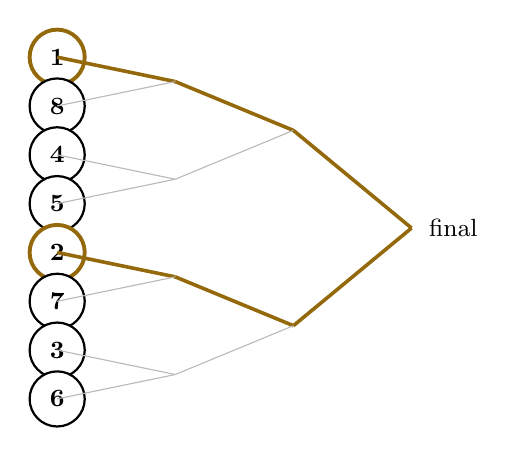
\begin{tikzpicture}[xscale=1.5,yscale=0.62]
  \def\seeds{{1,8,4,5,2,7,3,6}}
  % leaves
  \foreach \p in {0,...,7} {
    \pgfmathparse{\seeds[\p]}\edef\s{\pgfmathresult}
    \coordinate (l\p) at (0,-\p);
    \ifnum\p=0 \node[vtx,draw=brass,line width=1.4pt] at (l\p) {\s};
    \else\ifnum\p=4 \node[vtx,draw=brass,line width=1.4pt] at (l\p) {\s};
    \else \node[vtx] at (l\p) {\s};\fi\fi
  }
  % level 1 nodes
  \foreach \j in {0,...,3} { \coordinate (a\j) at (1, {-(2*\j+0.5)}); }
  % level 2 nodes
  \foreach \j in {0,1} { \coordinate (b\j) at (2, {-(4*\j+1.5)}); }
  % root
  \coordinate (root) at (3,-3.5);
  % edges leaves->level1
  \foreach \p in {0,...,7} { \pgfmathtruncatemacro{\j}{\p/2}
    \ifnum\p=0 \draw[brass,line width=1.3pt] (l\p)--(a\j);
    \else\ifnum\p=4 \draw[brass,line width=1.3pt] (l\p)--(a\j);
    \else \draw[gray!55] (l\p)--(a\j);\fi\fi }
  % level1->level2
  \foreach \j in {0,...,3} { \pgfmathtruncatemacro{\jj}{\j/2}
    \ifnum\j=0 \draw[brass,line width=1.3pt] (a\j)--(b\jj);
    \else\ifnum\j=2 \draw[brass,line width=1.3pt] (a\j)--(b\jj);
    \else \draw[gray!55] (a\j)--(b\jj);\fi\fi }
  % level2->root
  \draw[brass,line width=1.3pt] (b0)--(root);
  \draw[brass,line width=1.3pt] (b1)--(root);
  \node[right=1mm of root,font=\small] {final};
\end{tikzpicture}
\caption{The seeded eight player tree, seed order $[1,8,4,5,2,7,3,6]$. The paths of
seeds $1$ and $2$ (ringed) stay in opposite halves and meet only at the root, so
seeds $1$ and $2$ can meet only in the final.}
\label{fig:tree}
\end{figure}

The placement's fairness guarantee can be stated and proved exactly.

\begin{lemma}[Subtree isolation]
In the bracket built from $S(k)$, every subtree with $2^j$ leaves contains exactly
one of the top $k/2^j$ seeds.
\end{lemma}

\begin{proof}
Induct on the doubling. For $S(2) = [1,2]$ the claim is immediate. Assume it holds
for $S(m)$ and build $S(2m)$. The size two subtrees of the new bracket are exactly
the pairs $(s,\ 2m+1-s)$ with $s \in S(m)$, and since $s \le m < 2m+1-s$, each
contains exactly one of the top $m$ seeds; that is the $j=1$ case. Now contract
every pair to its smaller member. By construction this turns the $S(2m)$ bracket
into precisely the $S(m)$ bracket, and a subtree with $2^j$ leaves ($j \ge 1$)
contracts to one with $2^{j-1}$ leaves, which by the induction hypothesis contains
exactly one of the top $m/2^{j-1} = 2m/2^j$ seeds. The discarded partners all
exceed $m$, hence also $2m/2^j$, so the count is unchanged.
\end{proof}

Two players meet exactly when the knockout reaches the root of the smallest
subtree containing both, so the lemma pins down who can meet when: the top $2^t$
seeds occupy $2^t$ different subtrees of size $k/2^t$, hence no two of them can
meet before the round with $2^t$ players left. In particular seeds $1$ and $2$ can
meet only in the final, and seeds $1$ through $4$ no earlier than the semifinals.
The application computes the exact earliest meeting round as
\texttt{seedMeetRound}, the height of the two leaves' lowest common ancestor in
the tree. A single elimination of $k$ players is exactly $k-1$ matches, since each
match produces one loss and $k-1$ players must be eliminated once.

\subsection{Double elimination and the second life}

Single elimination is short and gives a clean tree, but one unlucky match, a bad
roll or a lost break, ends a strong player's run. Double elimination fixes this and
suits a casual event, because everyone plays more. Each player starts in the
winners bracket; a first loss drops them into the losers bracket, and a second loss
ends their run. So every player except the champion is eliminated with exactly two
losses. Figure~\ref{fig:de} shows the flow for four players.

\begin{figure}[h]
\centering
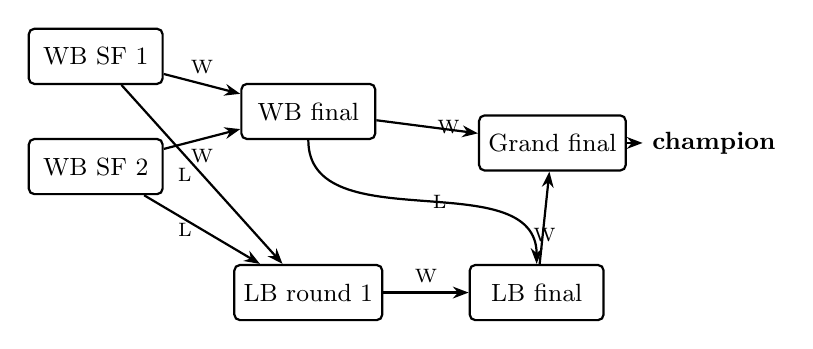
\begin{tikzpicture}
  \node[box] (sf1) at (0,0) {WB SF 1};
  \node[box] (sf2) at (0,-1.4) {WB SF 2};
  \node[box] (wf) at (2.7,-0.7) {WB final};
  \node[box] (lr1) at (2.7,-3.0) {LB round 1};
  \node[box] (lf) at (5.6,-3.0) {LB final};
  \node[box] (gf) at (5.8,-1.1) {Grand final};
  \node[right=2mm of gf,font=\small\bfseries] (ch) {champion};
  \draw[flow] (sf1) -- node[above,font=\scriptsize]{W} (wf);
  \draw[flow] (sf2) -- node[below,font=\scriptsize]{W} (wf);
  \draw[flow] (sf1) -- node[left,font=\scriptsize]{L} (lr1);
  \draw[flow] (sf2) -- node[left,font=\scriptsize]{L} (lr1);
  \draw[flow] (wf) -- node[right,font=\scriptsize]{W} (gf);
  \draw[flow] (wf) to[out=-90,in=90] node[right,font=\scriptsize]{L} (lf);
  \draw[flow] (lr1) -- node[above,font=\scriptsize]{W} (lf);
  \draw[flow] (lf) -- node[below,font=\scriptsize]{W} (gf);
  \draw[flow] (gf) -- (ch);
\end{tikzpicture}
\caption{Double elimination for $k=4$. A winners bracket (WB) loss (edge L) drops a
player into the losers bracket (LB); a second loss ends the run. The undefeated WB
champion meets the once beaten LB champion in the grand final.}
\label{fig:de}
\end{figure}

Counting by losses gives the totals directly. The $k-1$ non champions each carry two
losses, that is $2(k-1)$ losses, and the champion carries $0$ or $1$, so the number
of matches is
\[
2(k-1) + \{0 \text{ or } 1\} = \begin{cases} 2k-2 & \text{no reset}\\ 2k-1 & \text{grand final reset.}\end{cases}
\]
The reset arises because the WB champion enters the grand final undefeated: if the
LB champion wins the first grand final game, both then have one loss, so a single
deciding game is played. For $k=8$ this is $14$ or $15$ matches against $7$ for
single elimination. Table~\ref{tab:formats} summarizes the tradeoff.

\begin{table}[h]
\centering
\begin{tabular}{lcc}
\toprule
 & single elimination & double elimination \\
\midrule
eliminated after & $1$ loss & $2$ losses \\
matches for $k$ seeds & $k-1$ & $2k-2$ (reset: $2k-1$) \\
rounds for $k=8$ & $3$ & $8$ \\
minimum matches per player & $1$ & $2$ \\
survives one unlucky match & no & yes \\
\bottomrule
\end{tabular}
\caption{The knockout tradeoff. Double elimination roughly doubles the play and
guarantees every entrant at least two matches, at the cost of a longer event; the
application offers both, chosen with a format toggle.}
\label{tab:formats}
\end{table}

The construction \texttt{buildDoubleBracket} handles any $k = 2^m$. The winners
bracket is the ordinary seeded tree ($k-1$ matches). The losers bracket has
$2(m-1)$ rounds ($k-2$ matches) that alternate minor rounds, where losers bracket
survivors meet, and major rounds, where fresh winners bracket losers drop in. The
drops are crossed in reversed order, so a dropping player meets a survivor from the
opposite side of the draw rather than someone from their own quarter. This avoids
rematches for as long as the bracket is wide enough to permit it; once the losers
bracket narrows to single matches, rematches can occur, as in any double
elimination (for $k=4$ they are already unavoidable, since the losers final has
only one possible pairing). The whole bracket is built as a list of matches already
interleaved into a valid play order, each carrying a pointer to where its winner and
its loser go next, so a single match queue drives the simulation. For $k=8$ ($m=3$)
the losers bracket rounds hold $2, 2, 1, 1$ matches, six in all ($k-2$), so a full
run is $7$ winners bracket matches, $6$ losers bracket matches, and one grand final,
that is $14 = 2k-2$.

\section{A documented limitation: the carry-over effect}

If player $i$ faces $j$ in one round and $k$ in the next, then $k$ is said to
receive a \emph{carry-over} from $j$ through $i$, for example inheriting an opponent
who is tired or on a run. Reading each player's opponent sequence and wrapping the
last round to the first, one tallies the matrix $G$ where $G[j][k]$ counts these
handoffs, and measures imbalance by the sum of squares $\Gamma = \sum_{j,k} G[j][k]^2$.
A balanced schedule spreads the handoffs so every off diagonal entry is $1$,
reaching the minimum $\Gamma = n(n-1)$.

\begin{figure}[h]
\centering
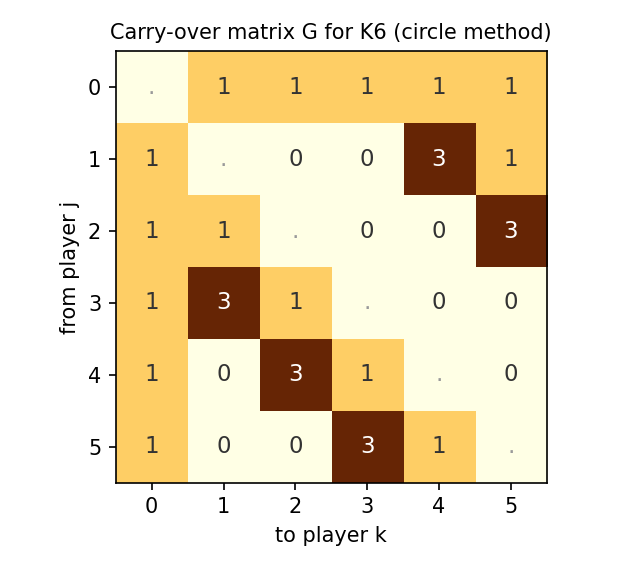
\includegraphics[width=0.44\textwidth]{report_carryover.png}
\caption{The carry-over matrix of the circle method schedule of $K_6$. The fixed
player (row $0$) hands off evenly, but the ring players concentrate into cells of
weight $3$. Its value is $\Gamma = 60$, exactly twice the balanced minimum
$n(n-1)=30$.}
\label{fig:carry}
\end{figure}

The circle method does the opposite of balancing. Russell (1980) showed a balanced
schedule exists whenever $n$ is a power of two, using finite field constructions,
while Lambrechts, Ficker, Goossens, and Spieksma (2018) proved that the circle
method attains the \emph{maximum} possible carry-over value, and that every schedule
achieving that maximum is a circle method schedule. So the very rotation that made
the round robin easy to build and prove is, provably, the least balanced choice for
carry-over. For a casual Student Union event the trade for simplicity is acceptable,
and the application states the limitation and draws the matrix live
(Figure~\ref{fig:carry}). This honesty, showing a weakness of the chosen method with
a citation, is itself part of the design.

The extremes are visible on small fields. For $n=4$ the complete graph $K_4$ has a
unique one-factorization, so the circle method has no freedom and its schedule is
already balanced: every off diagonal entry of $G$ is $1$ and $\Gamma = 12 = n(n-1)$,
the minimum. The gap between the circle method's maximum and the balanced minimum
opens only for $n \ge 6$, where the circle schedule of $K_6$ scores $\Gamma = 60$,
exactly twice the balanced minimum of $30$ (Figure~\ref{fig:carry}). Russell's
balanced designs, available whenever $n$ is a power of two, recover the minimum at
the cost of the simple rotation and its one line proof, which is the tradeoff a real
event has to weigh.

\section{Presenting the mathematics: the guided walkthrough}

Because the point of the project is the mathematics, the application does not just
use these results, it teaches them. A built in \emph{guided walkthrough} presents
the two core algorithms in eighteen steps across four acts (round robin, rating,
knockout tree, carry-over), each step pairing a short narration with a live
visual: the $K_6$ diagram inking one matching per rotation with chalk residue, the
congruence table of Table~\ref{tab:cong} computed from the shipped scheduler
(Figure~\ref{fig:walk}), the doubling seed order built pass by pass, the meeting
round highlighted on the tree, and the carry-over heatmap. The walkthrough runs on
a fixed teaching field, independent of the loaded roster, so it presents
identically every time, and it advances by button or arrow key, which is how the
ten minute live demonstration of this project is delivered: the walkthrough
carries the theory, and the live tournament run carries the practice.

\begin{figure}[h]
\centering
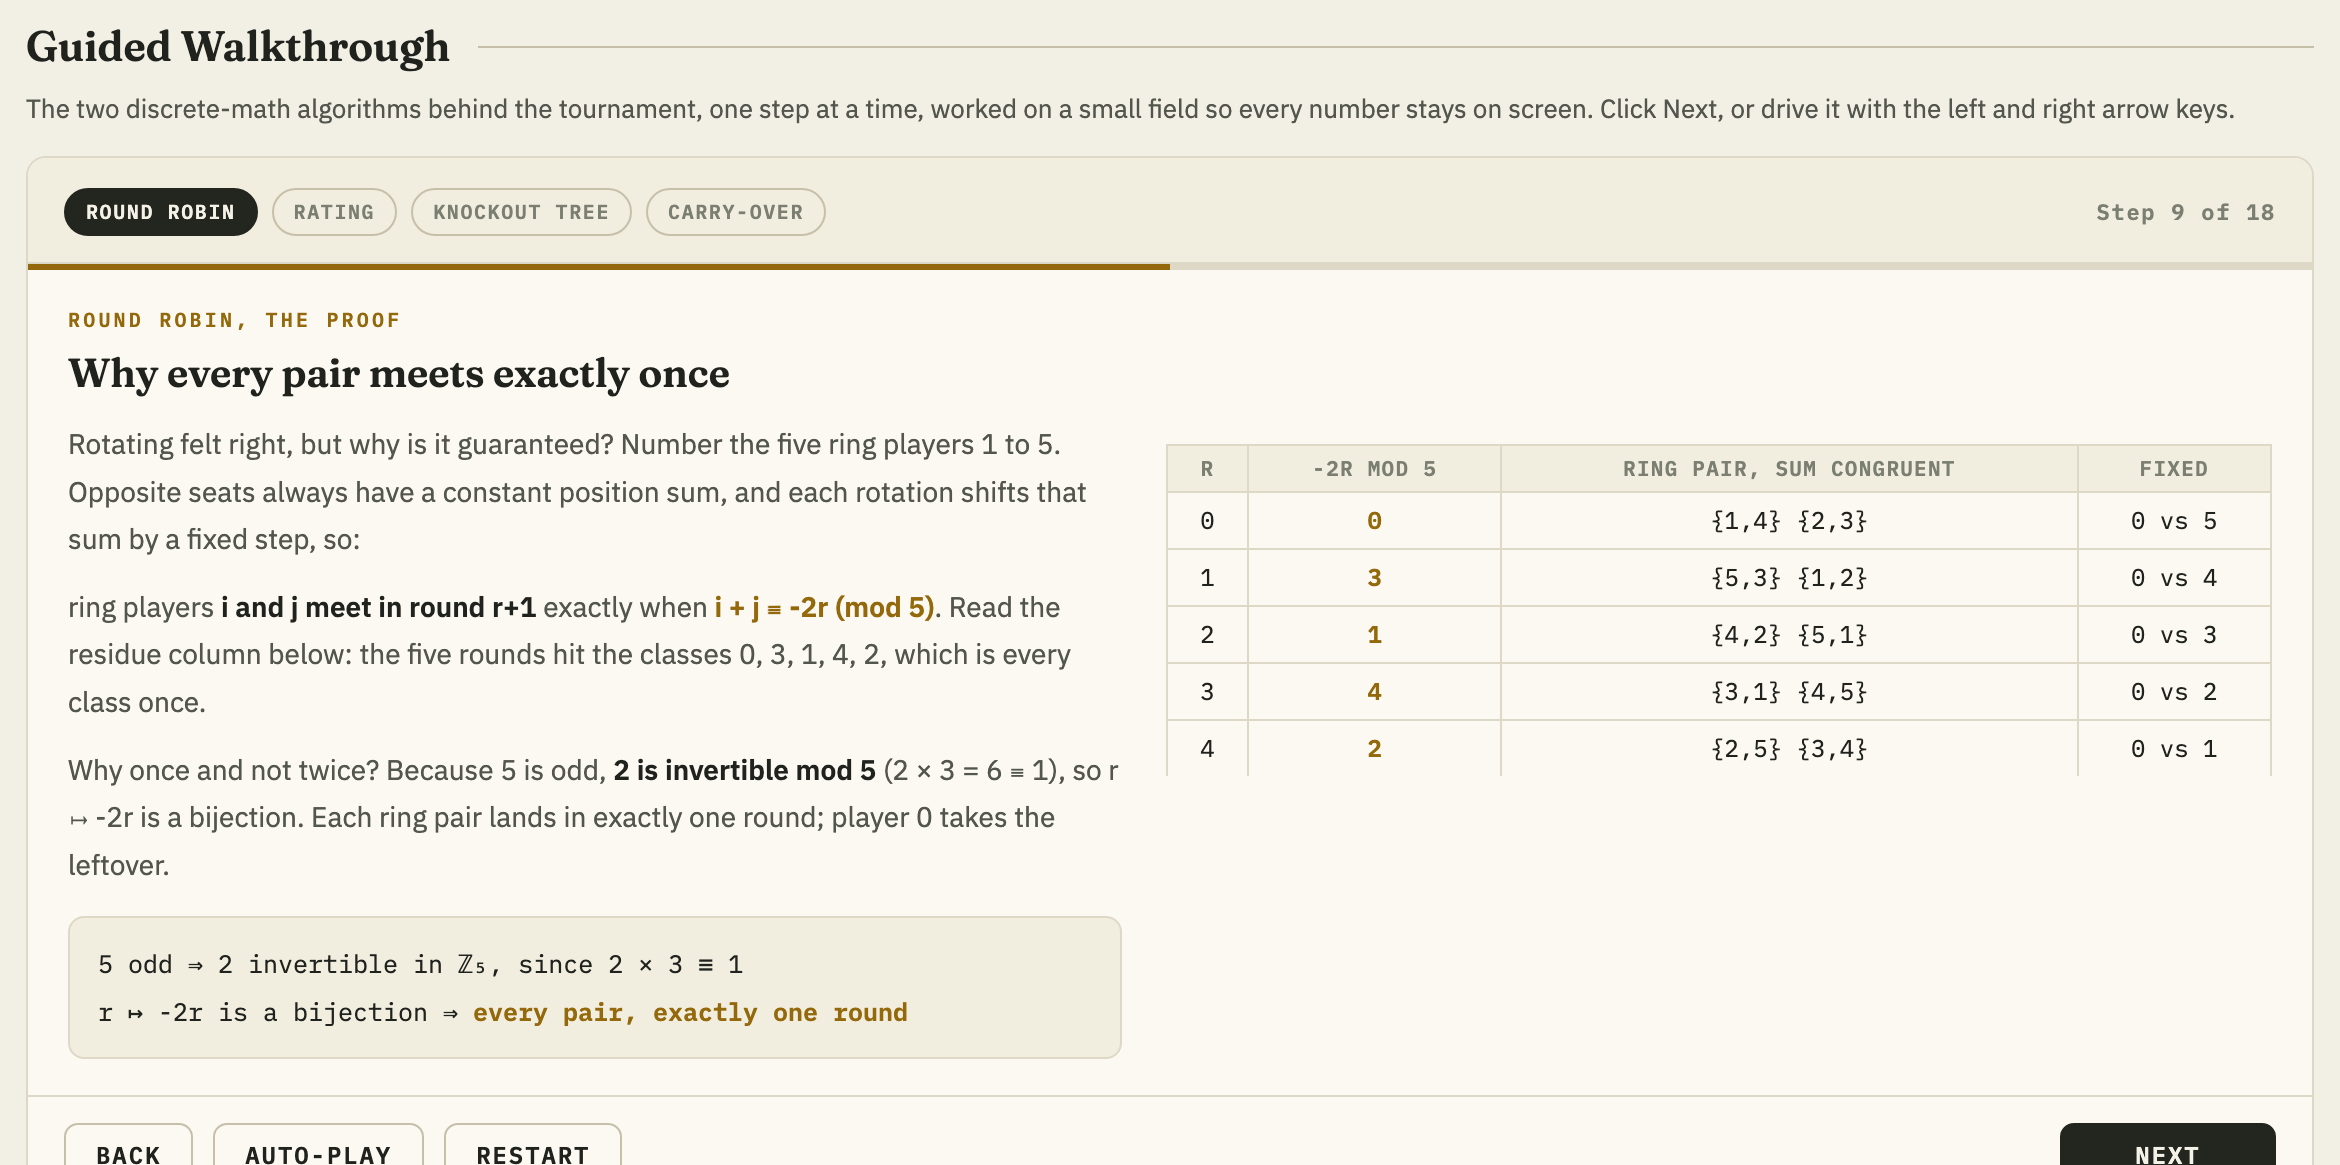
\includegraphics[width=0.97\textwidth]{report_walkthrough.png}
\caption{The walkthrough at the proof step of Act 1. The congruence table on the
right is generated live from the shipped \texttt{buildSchedule}, so the displayed
proof and the running code cannot disagree.}
\label{fig:walk}
\end{figure}

\section{Verification and results}

Correctness is established two ways. First, the application's algorithms live in a
DOM free block that a Node test runner extracts and exercises directly, so the
tested code is the shipped code. The suite runs roughly $108{,}000$ assertions: the
circle method's structure for every field size $n = 4$ to $30$, the congruence
invariant of Theorem 1, the Elo identities, the race inversion round trip and its
Monte Carlo, the seed order and meeting rounds, the carry-over totals, and full
simulated double eliminations that confirm the two loss invariant and the
$2k-2$ or $2k-1$ match count for $k = 4, 8, 16$. Second, the in application
verification panel recomputes the round robin's five structural properties from the
generated schedule on every run.

Figure~\ref{fig:app} shows a completed double elimination the application played
for a field of thirteen (top eight seeded). The run displays every piece of the
mathematics at once: the eighth seed upsets the first in the opening round, first
losses drop into the losers bracket and climb back through its alternating rounds,
the losers champion takes the first grand final game, and the reset game decides
the title, $15 = 2k-1$ matches in all. Fields up to thirty players keep every
guarantee: at $n=30$ the group stage is $29$ rounds and $435$ matches, all five
checks pass, and Elo is conserved.

The model also grounds the schedule in real time on real tables. Reading the
winner's score as exactly $N$ racks and the loser's as averaging $(N-1)/2$, a race
to $5$ runs about $7$ racks. At roughly eight minutes a rack on the Student Union's
six tables, with rounds played in waves when matches outnumber tables, the eight
player group stage comes to about six and a half hours of play, while the thirty
player field needs over eighty hours. The application displays this estimate beside
each schedule, which makes the practical scale of a live event visible: one long
evening fits a small field, and the thirty player tournaments in this report are
exactly the ones that can only be explored by simulation.

\begin{figure}[h]
\centering
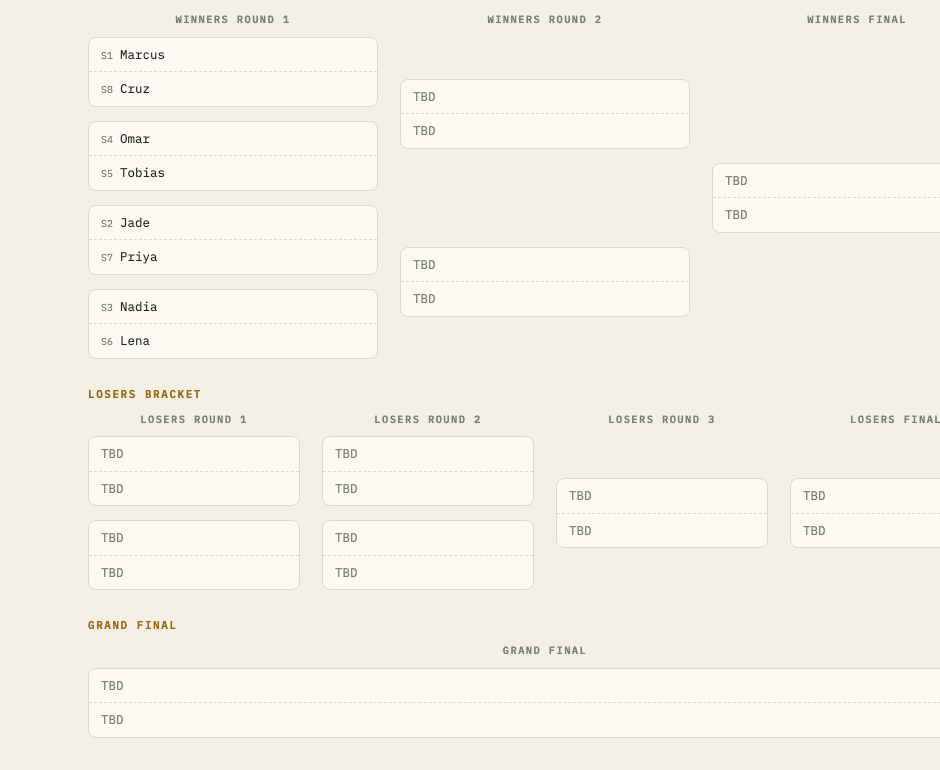
\includegraphics[width=0.94\textwidth]{report_de_bracket.png}
\caption{A completed double elimination in the application: the winners bracket
(the seeded tree), the losers bracket (six matches over four rounds for $k=8$),
and a grand final that went to the reset game.}
\label{fig:app}
\end{figure}

\section{Design decisions}

\begin{itemize}[nosep,leftmargin=1.4em]
  \item \textbf{Graph and one-factorization framing.} It turns vague scheduling into
        provable structure, which is the point of the course.
  \item \textbf{Circle method for the round robin.} The simplest construction with a
        short, fully rigorous proof. The honest cost is maximum carry-over, which the
        report and the app both state.
  \item \textbf{Calibrated race model over raw Elo as rack probability.} Keeps match
        odds faithful to ratings while producing realistic scorelines.
  \item \textbf{Both knockout formats.} Single elimination gives the clean binary
        tree for the mathematics; double elimination is fairer to one unlucky match
        and keeps everyone playing, which fits the event. Offering both makes the
        $k-1$ versus $2k-2$ tradeoff visible.
  \item \textbf{Live verification and an extracted test block.} Correctness is
        demonstrated from output, not asserted.
\end{itemize}

\section{What I learned}

The main lesson was how much of an apparently practical problem is really a question
about discrete structures, and how much that reframing pays off. Once who plays whom
became the edges of $K_n$, the schedule's correctness reduced to a one line fact
about modular arithmetic, and its fairness properties, byes and carry-over, became
theorems rather than guesses. I came to value constructions that arrive with proofs:
the circle method was chosen not because it is the only schedule (there are $6240$
for eight players) but because its correctness is short to state and to defend, which
matters when a professor can ask about it directly.

I also learned the discipline of showing a method's weakness. The carry-over result,
that my own chosen schedule is provably the worst for balance, was more convincing to
include than to hide, and stating it forced me to actually understand the tradeoff
rather than assume the method was ideal. Building the double elimination taught me to
think in invariants: instead of tracking a tangle of two brackets, the entire format
is pinned down by one counting argument, every non champion leaves with exactly two
losses, which both guided the implementation and became the property the tests check.
Finally, keeping the simulation honest to the ratings, by inverting the race formula
rather than reusing the Elo number, was a small reminder that a model can be subtly
wrong even when each piece looks right.

\section{Conclusion}

Behind a pool tournament sits a compact and provable core of discrete mathematics:
a one-factorization of $K_n$ built by a rotation that works because $2$ is a unit
modulo $n-1$, a chromatic index that explains byes, a negative binomial race
calibrated to Elo, seeded binary trees with an exact meeting distance, a loss
counting argument that pins down double elimination at $2k-2$ matches, and a
carry-over analysis in which the chosen method is provably extremal. The system
runs the tournament and, at every step, shows and checks the mathematics that makes
its decisions correct and fair.

\begin{thebibliography}{9}\small
\bibitem{kirkman} T. P. Kirkman, On a problem in combinations, \emph{Cambridge and Dublin Mathematical Journal} 2 (1847) 191-204.
\bibitem{lucas} \'E. Lucas, \emph{R\'ecr\'eations Math\'ematiques}, vol. 2, Gauthier-Villars, Paris, 1883.
\bibitem{russell} K. G. Russell, Balancing carry-over effects in round robin tournaments, \emph{Biometrika} 67 (1980) 127-131.
\bibitem{lam} E. Lambrechts, A. M. C. Ficker, D. R. Goossens, F. C. R. Spieksma, Round-robin tournaments generated by the circle method have maximum carry-over, \emph{Mathematical Programming} 172 (2018) 277-302.
\bibitem{elo} A. E. Elo, \emph{The Rating of Chessplayers, Past and Present}, Arco, 1978.
\bibitem{wallis} W. D. Wallis, \emph{One-Factorizations}, Kluwer, 1997.
\bibitem{vizing} V. G. Vizing, On an estimate of the chromatic class of a p-graph, \emph{Diskret. Analiz} 3 (1964) 25-30.
\bibitem{oeis} OEIS Foundation, Sequence A000438, Number of one-factorizations of $K_{2n}$.
\end{thebibliography}

\end{document}
